%\title{LaTeX Portrait Poster Template}
%%%%%%%%%%%%%%%%%%%%%%%%%%%%%%%%%%%%%%%%%
% a0poster Portrait Poster
% LaTeX Template
% Version 1.0 (22/06/13)
%
% The a0poster class was created by:
% Gerlinde Kettl and Matthias Weiser (tex@kettl.de)
% 
% This template has been downloaded from:
% http://www.LaTeXTemplates.com
%
% License:
% CC BY-NC-SA 3.0 (http://creativecommons.org/licenses/by-nc-sa/3.0/)
%
%%%%%%%%%%%%%%%%%%%%%%%%%%%%%%%%%%%%%%%%%

%----------------------------------------------------------------------------------------
%	PACKAGES AND OTHER DOCUMENT CONFIGURATIONS
%----------------------------------------------------------------------------------------
\documentclass[a0,portrait]{a0poster}
\usepackage{multicol} % This is so we can have multiple columns of text side-by-side
\columnsep=100pt % This is the amount of white space between the columns in the poster
\columnseprule=3pt % This is the thickness of the black line between the columns in the poster

\usepackage[svgnames]{xcolor} % Specify colors by their 'svgnames', for a full list of all colors available see here: http://www.latextemplates.com/svgnames-colors

\usepackage{times} % Use the times font
%\usepackage{palatino} % Uncomment to use the Palatino font

\usepackage{graphicx} % Required for including images
\graphicspath{{figures/}} % Location of the graphics files
\usepackage{booktabs} % Top and bottom rules for table
\usepackage[font=normalsize,labelfont=bf]{caption} % Required for specifying captions to tables and figures
\usepackage{amsfonts, amsmath, amsthm, amssymb} % For math fonts, symbols and environments
\usepackage{wrapfig} % Allows wrapping text around tables and figures
\usepackage{natbib}
\bibliographystyle{apalike}
\newcommand{\jri}[1]{\textcolor{blue}{ \emph{\scriptsize  #1}} }

\begin{document}
%----------------------------------------------------------------------------------------
%	POSTER HEADER 
%----------------------------------------------------------------------------------------

% The header is divided into two boxes:
% The first is 75% wide and houses the title, subtitle, names, university/organization and contact information
% The second is 25% wide and houses a logo for your university/organization or a photo of you
% The widths of these boxes can be easily edited to accommodate your content as you see fit
%
\begin{minipage}[b]{0.15\textwidth}

\includegraphics[width=10cm]{cornkey.png}\\
%
\includegraphics[width=5cm]{pslogo.jpg}\\
\end{minipage}
%
\begin{minipage}[b]{0.7\textwidth}
\Huge \color{NavyBlue} \textbf{Utilizing Evolutionary Conservation Information to \\ Improve Prediction Accuracy in Genomic Selection} \color{Black}\\[0.5cm] % Title
%\Huge\textit{An Exploration of Complexity}\\[2cm] % Subtitle
\Large \textbf{Jinliang Yang$^1$, Sofiane Mezmouk$^{1,2}$, Rita Mumm$^3$, and Jeffrey Ross-Ibarra$^1$ }\\[0.5cm] % Author(s)
\large $^1$Department of Plant Sciences, University of California, Davis, CA 95616, USA \\%[0.4cm] % University/organization
\large $^2$Current address: KWS SAAT AG, Grimsehlstr. 31, 37555 Einbeck, Germany \\ %[0.4cm] % University/organization
\large $^3$Department of Crop Sciences, University of Illinois at Urbana-Champaign, Urbana, IL 61801, USA \\[0.4cm] % University/organization
%\Large \texttt{john@LaTeXTemplates.com} --- 1 (000) 111 1111\\
\end{minipage}
%
\begin{minipage}[b]{0.15\textwidth}

\includegraphics[width=10cm]{pslogo.jpg}\\
\end{minipage}
%


\vspace{1cm} % A bit of extra whitespace between the header and poster content

%----------------------------------------------------------------------------------------

\begin{multicols}{2} % This is how many columns your poster will be broken into, a portrait poster is generally split into 2 columns

%----------------------------------------------------------------------------------------
%	ABSTRACT
%----------------------------------------------------------------------------------------

\color{Navy} % Navy color for the abstract

\section*{ABSTRACT}
Genomic selection (GS) has gained popularity recently as the availability of genome-wide markers has increased. Current methods for GS weigh all the available SNPs equally in model training, without considering their functional differences. Genetic variations detected at evolutionary conserved sites tend to be deleterious and, thus, may be more informative for GS. To utilize this kind of information as a prior into the GS model, we proposed a method to put more weight on evolutionarily constrained sites. As a proof-of-concept, a half diallel population based on 12 diverse inbred lines was used, from which seven phenotypic traits were collected. Some of these traits show high levels of heterosis. After sequencing the 12 founder lines, about 14 million SNPs were discovered and the SNPs were used to identify 502,913 haplotype blocks shared through identity by descent (IBD). A five fold cross-validation experiment was conducted using the summary statistics of the SNP conservation scores, which were computed by evaluating sequences similarity of multiple divergent species, in the IBD blocks as explanatory variables. The results show that the prediction accuracies are significantly better than shuffled data with randomly assigned conservation scores. This study demonstrates the importance of incorporating evolutionary information in GS and its potential use in plant breeding.


%----------------------------------------------------------------------------------------
%	INTRODUCTION
%----------------------------------------------------------------------------------------

\color{SaddleBrown} % SaddleBrown color for the introduction

\section*{Objectives}
\begin{itemize}
\item Study deleterious variants in a maize diallel population and their contributions to heterosis.
\item Quantify IBD blocks by using evolutionary conservation information.
\item Test whether it is useful to incorporate evolutionary conservation information in genomic selection.
\end{itemize}

%----------------------------------------------------------------------------------------
%	MATERIALS AND METHODS
%----------------------------------------------------------------------------------------

\section*{Materials and Methods}

\subsection*{Plant materials and phenotypic data}
%-------------------
%Figure
\begin{center}\vspace{1cm}
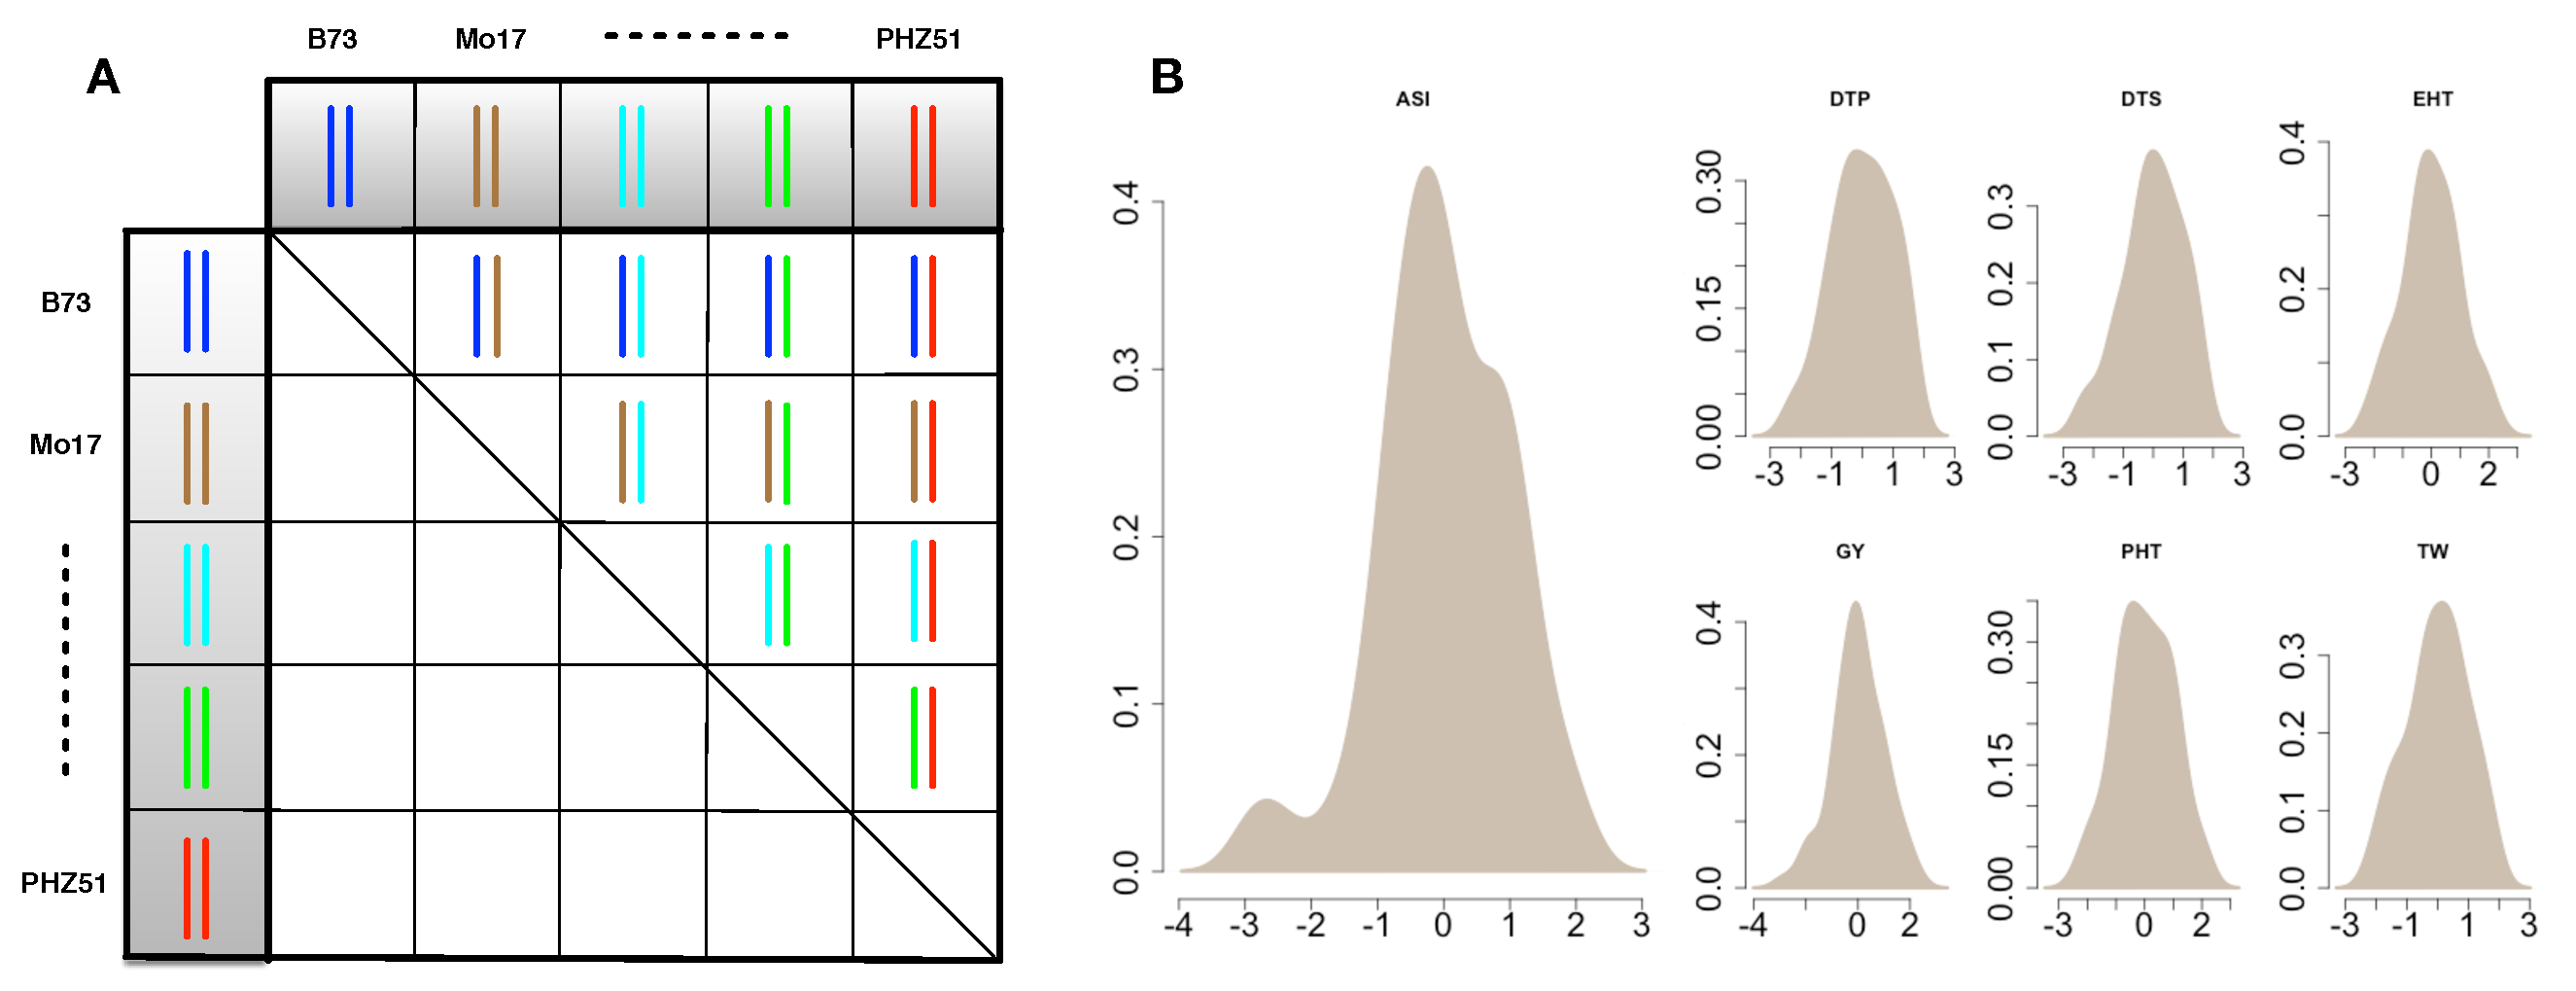
\includegraphics[width=0.8\linewidth]{pvp.pdf}
\captionof{figure}
{\color{black} \textbf{Diallel experimental design and distribution of phenotypic data.}
\textbf{(A)} Twelve maize inbred lines were selected and crossed in a half diallel. Ten of these (LH1, LH123HT, LH82, PH207, 4676A, PHG39, PHG47, PHG84, PHJ40, PHZ51) are proprietary inbreds that have expired from Plant Variety Protection (PVP) and represent the lineage of key heterotic germplasm pools used in present-day commercial corn hybrids. Two of them are important public inbreds, B73 and Mo17. \textbf{(B)} Phenotypic data were collected for anthesis-silking interval (ASI, in days), days to 50\% pollen shed (DTP), days to 50\% silking (DTS), ear height (EHT, in cm), grain yield adjusted to 15.5\% moisture (GY, in bu/A), plant height (PHT, in cm), and test weight (TW, in pounds). Analyses were carried out on the traits per se as well as percent high parent heterosis (pHPH).
}
\end{center}\vspace{1cm}

\subsection*{Sequencing and SNP conservation annotation}
%------------------
% wet lab
All twelve inbreds were sequenced to an average depth of $\sim$10X. Reads were mapped to the maize B73 reference genome (AGPv2) with bwa-mem.  After filtering, 13.8M SNPs were kept for further comparisons, including 1.9M genic SNPs and 361,280 in protein coding regions. Genome-wide deleterious variants were characterized by using genomic evolutionary rate profiling (GERP) \citep{Davydov2010}. %\jri{bibliography style can be extremely short. no need to list title, all authors, etc.}

\begin{center}\vspace{1cm}
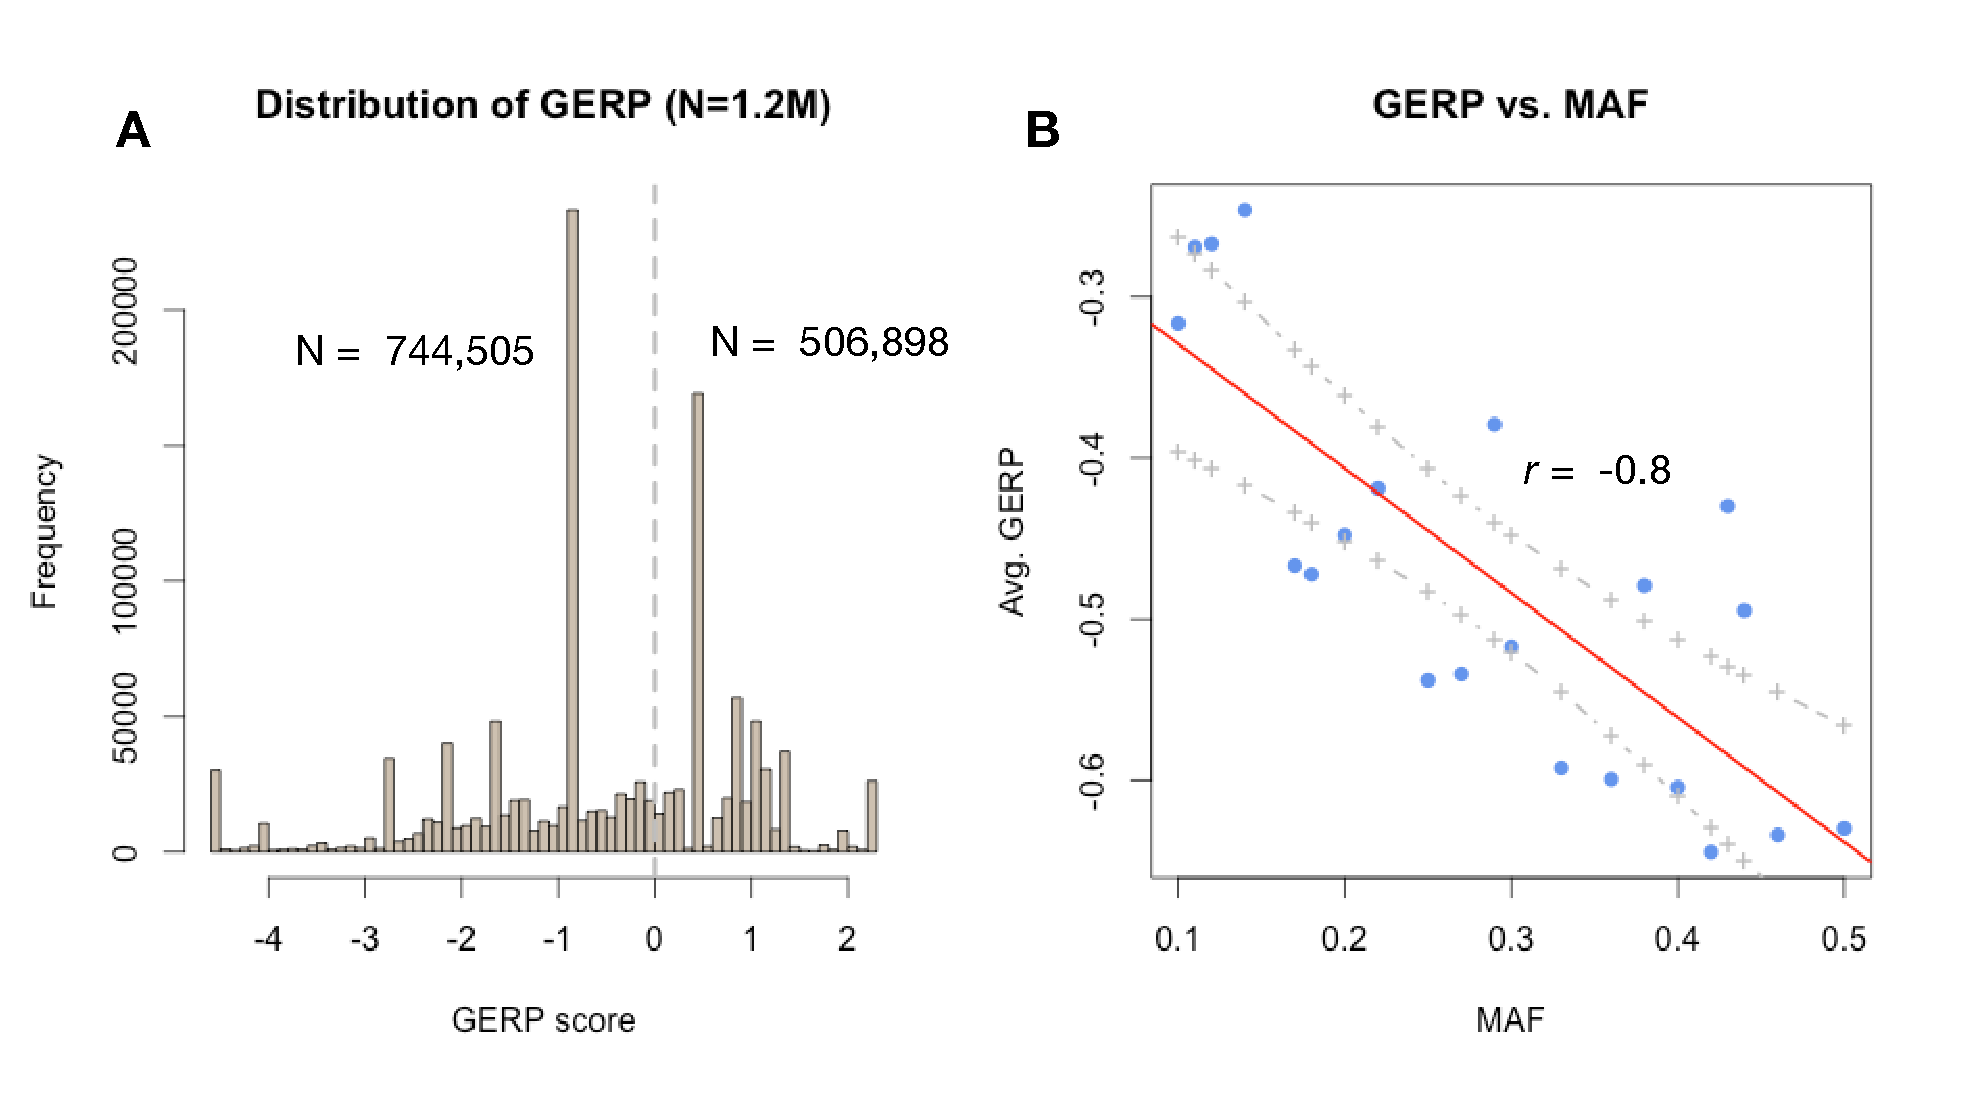
\includegraphics[width=0.8\linewidth]{gerp.pdf}
\captionof{figure}{
\color{black} \textbf{GERP distribution of SNPs and relationship between GERP and minor allele frequency.}
\textbf{(A)} GERP scores were obtained for $\sim$1.2 million ($\sim$10\%) SNPs. Of these, 506,898 (42\%) were under evolutionary constraint and considered as deleterious variants. 
\textbf{(B)} Mean GERP scores were calculated for each bin (bin size = 0.01) of minor allele frequency (MAF) shows that variants at conserved sites are maintained at low frequency. The red line and grey lines define the regression and its 95\% confidence interval.}
\end{center}\vspace{1cm}

%----------------------------------------------------------------------------------------
%    ACKNOWLEDGEMENTS
%----------------------------------------------------------------------------------------
\color{DarkSlateGray}
\section*{Acknowledgements}

Funding for this project comes from the USDA-AFRI, USDA Hatch, DuPont Pioneer, and N2 Genetics. We would like to thank Eli Rodgers-Melnick for allowing us to use his GERP rate estimations. 


%Figure GERP IBD
\color{SaddleBrown}
\subsection*{Computing conservation score for IBD blocks}
%------------------

\begin{center}\vspace{1cm}
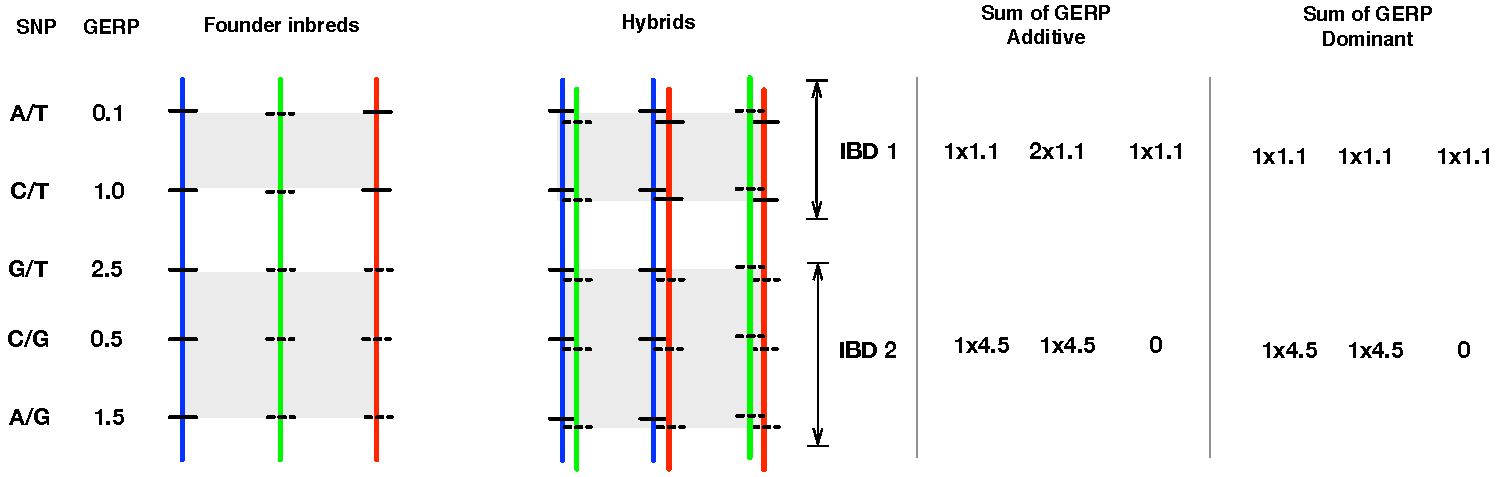
\includegraphics[width=1\linewidth]{gerpIBD.pdf}
\captionof{figure}{
\color{black} \textbf{Incoporation of conservation information into IBD blocks.}
Regions of the genome that are identical by descent (IBD) among the 12 inbreds were identified using Beagle \citep{Browning2009}.  The GERP scores of SNPs in an IBD block were summed under both additive and dominant models. Under the additive model, 2 x GERP score was assigned to genotypes homozygous for the non-reference allele, 1 x GERP score was assigned to heterozygotes, and 0 was assigned to the homozygous reference genotype. Under the dominant model, 1 x GERP score was assigned to both genotypes with a nonreference allle and 0 to the homozygous reference genotype.}
\end{center}\vspace{1cm}

\subsection*{Genomic selection models}

A Bayesian-based approach (BayesC) \citep{Habier2011} was employed for the genomic selection (GS) experiments. To estimate predict accuracies, the diallel population was randomly divided into training and validation sets for 10 times using a 5-fold cross-validation method. Circular permutations were used both considering all SNPs or considering only genic SNPs to control for differences between genic and nongenic regions.

%----------------------------------------------------------------------------------------
%	RESULTS 
%----------------------------------------------------------------------------------------


\section*{Results}

For traits \emph{per se}, model prediction accuracies were significantly improved for ASI, DTS and PHT when incorporating GERP score information under the additive model. Prediction accuracies were significantly improved for ASI, DTP, GY and TW under the dominant model. In general, the average prediction rates are higher using the additive model (\emph{r} = 0.8) than the dominant model (\emph{r} = 0.7). For heterosis, incorporation of GERP scores only improved grain yield prediction and only under a dominant model.  

\begin{center}\vspace{1cm}
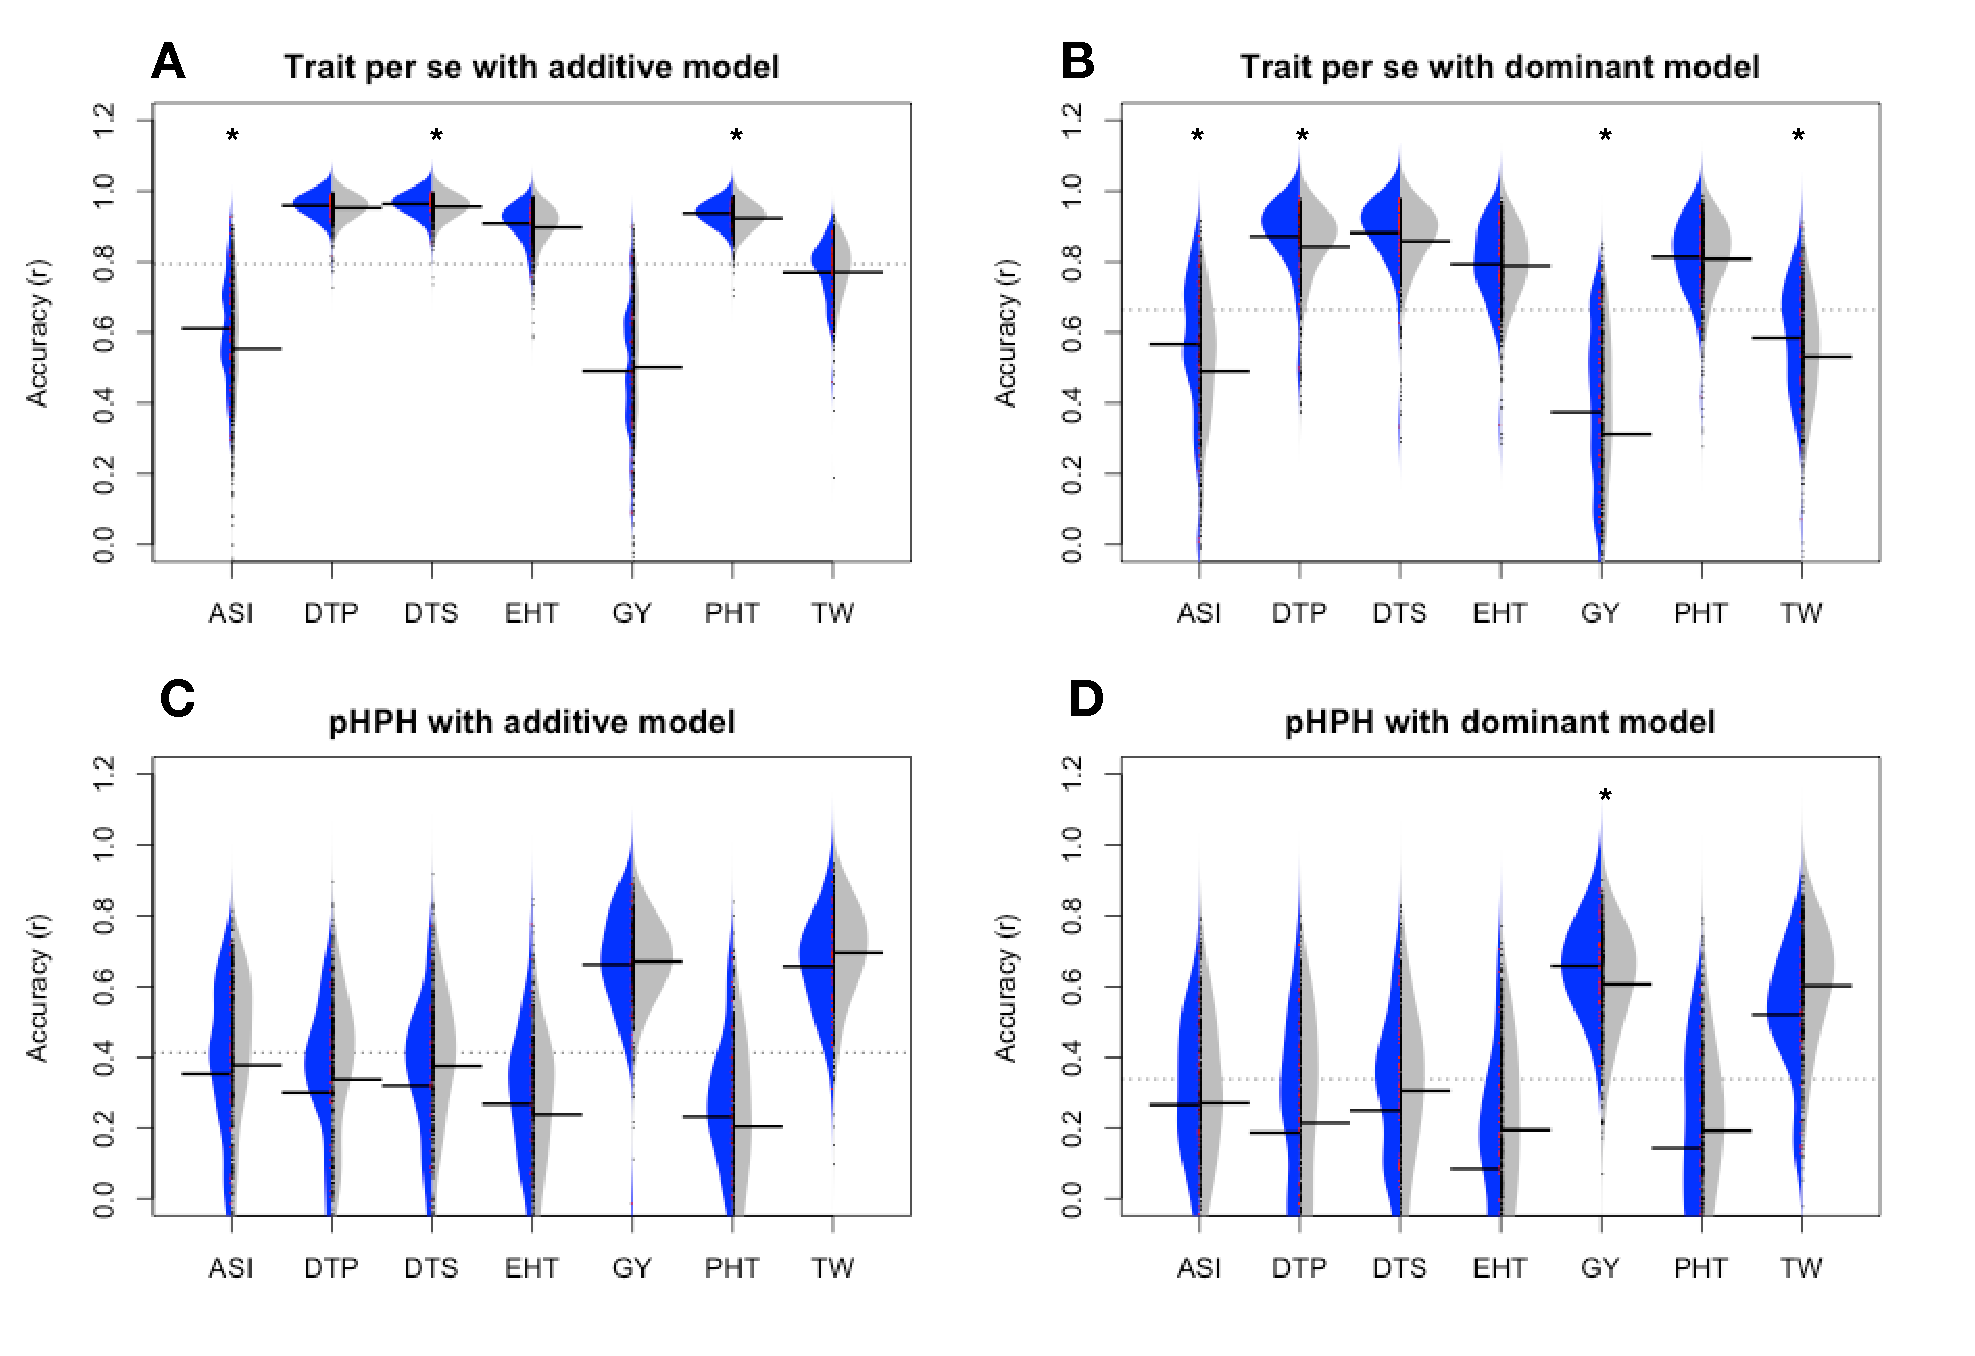
\includegraphics[width=0.8\linewidth]{cvres.pdf}
\captionof{figure}{
\color{black} \textbf{Beanplots of cross-validation accuracies.}
Cross-validation experiments were conducted using genic SNPs and circular shuffled data from the same set of the genic SNPs for traits \emph{per se} (\textbf{A, B}) and pHPH (\textbf{C, D}) under additive (\textbf{A, C}) and dominant (\textbf{B, D}) models. Accuaries from the real data were plotted on the left side of the bean (blue) and permutation results plotted on the right (grey). Horizotal bars on beans indicate mean accuracies. The grey dashed line indicates the overall average accuracy. Stars indicate significantly improved cross-validation accuracies.
}
\end{center}\vspace{1cm}

%----------------------------------------------------------------------------------------
%	CONCLUSIONS
%----------------------------------------------------------------------------------------

\color{SaddleBrown} % SaddleBrown color for the conclusions to make them stand out

\section*{Conclusions}

\begin{itemize}
\item More than 500,000 deleterious SNPs were identified in elite maize lines including in noncoding regions of the genome.
\item A genomic selection pipeline was developed, which utilized evolutionary conservation information in the model.
\item Cross-validation results suggested prediction accuracies for some traits could be significantly improved by incorporating GERP scores. 
\end{itemize}

\color{DarkSlateGray} % Set the color back to DarkSlateGray for the rest of the content

%----------------------------------------------------------------------------------------
%	FORTHCOMING RESEARCH
%----------------------------------------------------------------------------------------

%\section*{Forthcoming Research}

%----------------------------------------------------------------------------------------
%	REFERENCES
%----------------------------------------------------------------------------------------

%\nocite{*} % Print all references regardless of whether they were cited in the poster or not
%\bibliographystyle{plain} % Plain referencing style
\bibliography{sample} % Use the example bibliography file sample.bib


%----------------------------------------------------------------------------------------

\end{multicols}
\end{document}